\section{Dwarfs of computing}
\begin{itemize}
    \item Dense linear algebra
    \item Sparse linear algebra
    \item Spectral methods
    \item N-body methods
    \item Structured grids
    \item Unstructured grids
    \item Monte Carlo methods
    \item MapReduce
    \item Combinational Logic
    \item Dynamic Programming
    \item Graph Traversal
    \item BackTracking and Branch and Bound
    \item Graphical Models
    \item Finite State Machine
\end{itemize}

\subsection{Dense linear algebra}
Problems can be Categorized based on scaling of operations vs. data volume as below:
\begin{itemize}
    \item BLAS level 1 ($ O(n) $)
        \\ Dot product, scale, copy, \dots
    \item BLAS level 2 ($ O(n^2) $)
        \\ $ Matrix \times Vector $, convolution, \dots
    \item BLAS level 3 ($ O(n^3) $)
        \\ $ Matrix \times Matrix $, dense eigenvalue solvers, matrix inversion, \dots
\end{itemize}

Existing implementations and libraries
\begin{itemize}
    \item BLAS, LAPACK
        \begin{itemize}
            \item Naïve implementations on netlib.org
            \item Vendor-optimized, shared-memory parallel implementations available (e.g., MKL, CUDABlas)
        \end{itemize}
    \item SCALAPACK
        \begin{itemize}
            \item Distributed-memory parallel LAPACK (netlib.org)
            \item Available, e.g., in Cluster MKL
        \end{itemize}
\end{itemize}

\subsection{Sparse linear Algebra}
“\verb|Sparse|”: $ N \times N $ Matrices have $ O(N) $ nonzero entries

\paragraph{Typical operation:} Sparse $ Matrix \times Vector $

Used in sparse eigenvalue solvers and solvers for systems of linear equations
\begin{itemize}
    \item Store only $ N_{nz} $ nonzero elements of matrix and RHS, LHS vectors
    \item with $ N_r $ (number of matrix rows) entries
    \item “Sparse”: $ N_{nz} ~ N_r $
    \item Type $ O(N)/O(N) \implies \text{memory bound} $ \footnote{Nevertheless, there is more than one loop here!}
\end{itemize}

\begin{figure}[!htbp]
    \centering
    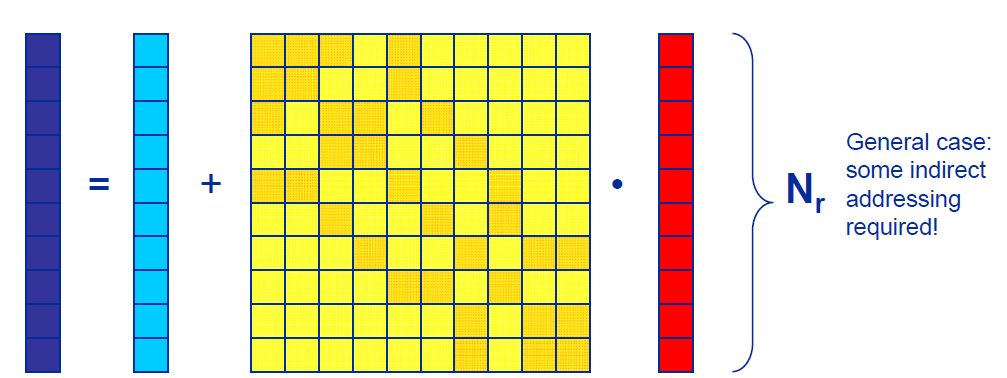
\includegraphics[width=0.7\textwidth]{sMvM}
    \caption{Sparse matrix-vector multiply (sMVM)}
\end{figure}

\subsection{Spectral methods}
\begin{itemize}
    \item $ O(N log N)/O(N) $
    \item Standard high performance implementation: FFTW
    \item MKL: Shared-memory parallel versions
    \item GPU: CUFFT
\end{itemize}
\begin{figure}[!htbp]
    \centering
    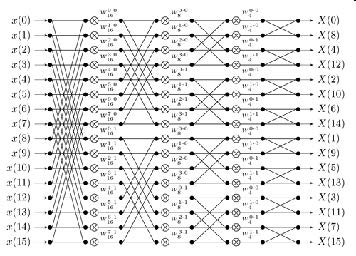
\includegraphics[width=0.7\textwidth]{spectral-methods}
    \caption{Spectral Method}
\end{figure}

\subsection{N-body methods}
Interactions between discrete points, not necessarily short-ranged i.e. Gravitational N-body

\paragraph{In general} $ O(N^2)/O(N) $
Optimizations/approximations possible are: 
\begin{itemize}
    \item Mean-field (Barnes-Hut, fast multipole, particle-in-cell) $ \implies O(N log N)/O(N) $
    or even $ O(N)/O(N) $
    \item Short-range interactions: $ \implies O(N)/O(N) $
\end{itemize}

\begin{figure}[!htbp]
    \centering
    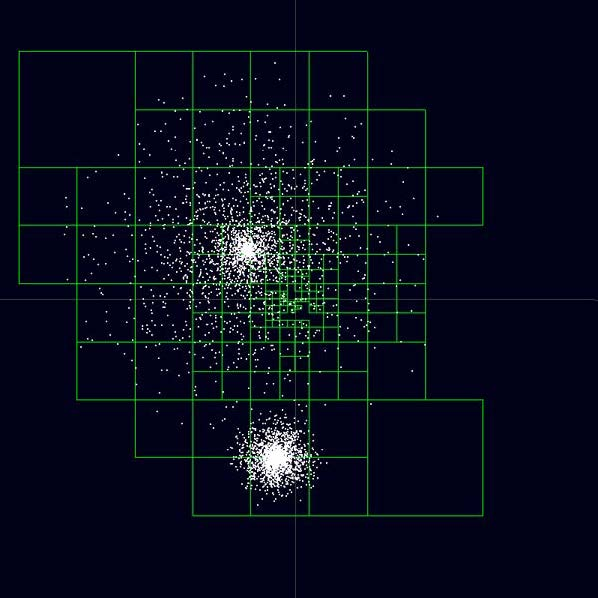
\includegraphics[width=0.7\textwidth]{n-body}
    \caption{N-body}
\end{figure}


\subsection{Structured grids}
\begin{itemize}
    \item Physical problem mapped to regular grid
    \item At the core of many PDE solvers
    \item \textbf{Simple relaxation methods:} Jacobi, Gauss-Seidel
    \item “Sweeps” are performed to update lattice sites
    \item Multigrid: Use successive grid coarsening and refinement to accelerate convergence
\end{itemize}

\begin{figure}[!htbp]
    \centering
    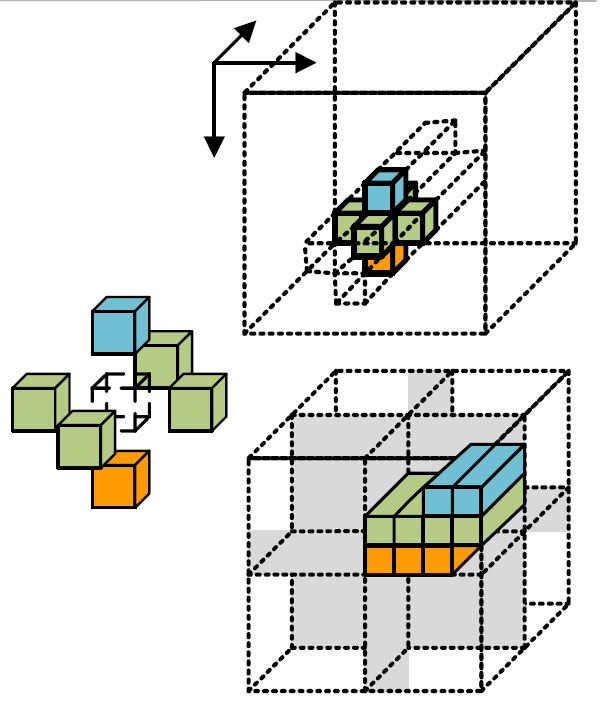
\includegraphics[width=0.7\textwidth]{structured-grids}
    \caption{Structured Grids}
\end{figure}

\subsection{Unstructured grids}
\begin{itemize}
    \item Irregular lattice, probably varying number of neighbors
    \item Neighbor relations must be explicitly stored
    \item Highly indirect data access patterns
\end{itemize}

\begin{figure}[!htbp]
    \centering
    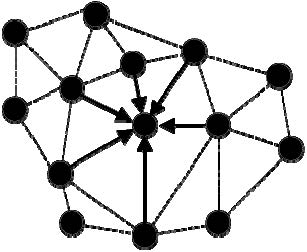
\includegraphics[width=0.7\textwidth]{unstructured-grids}
    \caption{Unstructured Grids}
\end{figure}

\subsection{Monte Carlo methods}
\begin{itemize}
    \item Computations by statistical sampling
    \item often used to cover “integration space” which would otherwise be too large to scan by brute force
    \item embarrassingly parallel
    \item Random number generation may be a bottleneck
\end{itemize}


\begin{figure}[!htbp]
    \centering
    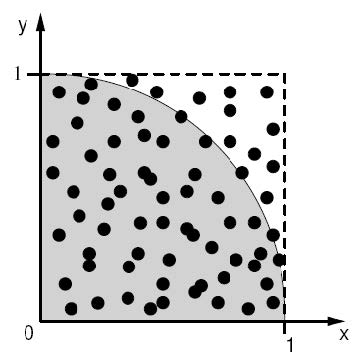
\includegraphics[width=0.7\textwidth]{monte-carlo}
    \caption{Monte Carlo methods}
\end{figure}

